\documentclass[11pt,a4paper]{article}
\usepackage[utf8]{inputenc}
\usepackage[T1]{fontenc}
\usepackage{babel}
\renewcommand{\contentsname}{Table des mati\`eres}
\usepackage{lmodern}
\usepackage[margin=2cm]{geometry}
\usepackage{xcolor}
\usepackage{titlesec}
\usepackage{longtable}
\usepackage{booktabs}
\usepackage{colortbl}
\usepackage{graphicx}
\usepackage{parskip}
\usepackage{hyperref}

\definecolor{navy}{HTML}{111111}
\definecolor{gold}{HTML}{1565C0}
\definecolor{greytext}{HTML}{555555}
\definecolor{lightgrey}{HTML}{F2F4F9}

\titleformat{\section}{\Large\bfseries\color{navy}}{\thesection}{0.6em}{}[{\color{navy}\titlerule}]
\titleformat{\subsection}{\large\bfseries\color{gold}}{\thesubsection}{0.6em}{}

\hypersetup{colorlinks=true, linkcolor=navy, urlcolor=navy, citecolor=navy}

\newcommand{\tblhead}[1]{\textcolor{white}{\textbf{#1}}}

% Encadre de mise a jour (ajoute le 03/09/2026) : ce document est la fiche de
% cadrage d'origine (redigee le 7 juillet 2026), volontairement conservee telle
% quelle -- chaque encadre \majcadrage signale, a l'endroit concerne, ce qui a
% reellement change depuis et pourquoi, sans reecrire le plan initial.
\newcommand{\majcadrage}[1]{%
\par\vspace{0.35cm}
\noindent\colorbox{lightgrey}{%
\begin{minipage}{\dimexpr\linewidth-2\fboxsep}
\vspace{0.15cm}
\textbf{\color{gold}Mise \`a jour (03/09/2026) :} #1
\vspace{0.15cm}
\end{minipage}%
}
\vspace{0.35cm}
}

\begin{document}

\begin{titlepage}
\centering
\vspace*{2cm}
{\Huge\bfseries\color{navy} Fiche de cadrage d\'etaill\'ee\par}
\vspace{0.5cm}
{\Large\bfseries\color{gold} Syst\`eme de questions-r\'eponses (RAG) pour le site institutionnel hcp.ma\par}
\vspace{1.5cm}
{\large\color{greytext} Structure d'accueil~: Haut-Commissariat au Plan (HCP), Direction des Syst\`emes d'Information Statistiques\par}
\vspace{0.3cm}
{\large\color{greytext} Bin\^ome~: Ayman El Baida et Saad Mesbah\par}
\vspace{0.3cm}
{\large\color{greytext} P\'eriode du stage~: 1er juillet -- fin ao\^ut 2026\par}
\vspace{0.3cm}
{\large\itshape\color{greytext} Document r\'edig\'e le 7 juillet 2026 -- support pour le rapport de stage et la communication du projet\par}
\vfill
\end{titlepage}

\tableofcontents
\newpage

\section{Pr\'esentation de l'organisme d'accueil}
Le Haut-Commissariat au Plan (HCP) est l'institution marocaine charg\'ee de la production statistique officielle, de la planification, de la prospective, de l'analyse et de la pr\'evision \'economique du Royaume du Maroc. Ses domaines de comp\'etence couvrent notamment la d\'emographie et les recensements g\'en\'eraux de la population et de l'habitat (le dernier RGPH, r\'ealis\'e en 2024, d\'enombrant une population l\'egale de 36~828~330 habitants), les comptes nationaux et la conjoncture \'economique, le march\'e du travail (activit\'e, emploi, ch\^omage), les indices des prix et de la production, le suivi des objectifs de d\'eveloppement durable (ODD), et le nouveau mod\`ele de d\'eveloppement.

Le stage se d\'eroule au sein de la Direction des Syst\`emes d'Information Statistiques, la direction en charge de l'infrastructure num\'erique et de la valorisation technologique des donn\'ees produites par le HCP -- un positionnement particuli\`erement pertinent pour un projet d'intelligence artificielle appliqu\'e \`a la diffusion de l'information statistique officielle.

\section{Nature et p\'erim\`etre du projet}
Ce projet s'inscrit dans le cadre d'un stage men\'e au sein de la Direction des Syst\`emes d'Information Statistiques du HCP. Il s'agit d'un projet de recherche appliqu\'ee visant \`a concevoir et d\'evelopper un prototype fonctionnel de syst\`eme de question-r\'eponse fond\'e sur la g\'en\'eration augment\'ee par r\'ecup\'eration (Retrieval-Augmented Generation, RAG), exploitant le contenu du site institutionnel hcp.ma. Le projet est men\'e en bin\^ome, sur une dur\'ee resserr\'ee de 4 \`a 8 semaines, avec un objectif de livraison d'un prototype d\'emontrable d\'ebut ao\^ut et une marge de s\'ecurit\'e jusqu'\`a fin ao\^ut.

\subsection{P\'erim\`etre retenu}
\begin{itemize}
\item Contenu source~: s\'election cibl\'ee de cat\'egories du site (publications et notes d'information des rubriques \'Economie, March\'e du travail, Population \& d\'emographie~; glossaire «~Concepts et d\'efinitions~»~; foire aux questions~; un ensemble curat\'e d'indicateurs cl\'es -- ch\^omage, inflation, PIB, population).
\item Langue~: fran\c{c}ais en priorit\'e pour le prototype~; l'arabe est une extension possible si le calendrier le permet.
\item Utilisateurs cibl\'es~: con\c{c}u pour le grand public visiteur de hcp.ma, transposable \`a un usage interne aux agents du HCP.
\item Livrable attendu~: un prototype fonctionnel document\'e, accompagn\'e d'une \'evaluation de fiabilit\'e.
\end{itemize}

\majcadrage{Le projet a finalement \'et\'e men\'e en solo par Ayman El Baida, et non en bin\^ome comme pr\'evu \`a la page de titre de ce document (r\'edig\'ee le 7 juillet, refl\'etant la situation de d\'epart). Voir le rapport de stage pour le d\'etail.}

\subsection{Hors p\'erim\`etre pour cette premi\`ere it\'eration}
\begin{itemize}
\item Crawl exhaustif de l'int\'egralit\'e du site hcp.ma.
\item Support arabe complet d\`es la premi\`ere version.
\item Infrastructure de production s\'ecuris\'ee ou h\'ebergement souverain on-premise.
\item Int\'egration dans les applications web dynamiques existantes (comptes nationaux, simulateurs, r\'esultats RGPH 2024).
\end{itemize}

\section{Contexte et probl\'ematique}
Le site hcp.ma centralise un volume important d'informations statistiques officielles, mais sous des formats h\'et\'erog\`enes~: pages HTML \'editoriales, documents PDF souvent bilingues (fran\c{c}ais/arabe), glossaire de concepts, foire aux questions, et donn\'ees chiffr\'ees structur\'ees (indicateurs, s\'eries temporelles, micro-donn\'ees). Un usager -- citoyen, chercheur, journaliste ou agent du HCP -- qui cherche une information pr\'ecise doit aujourd'hui naviguer manuellement dans cette architecture ou utiliser une recherche par mots-cl\'es, laquelle ne comprend pas les questions formul\'ees en langage naturel et ne permet pas de croiser plusieurs sources pour construire une r\'eponse.

Un chatbot fond\'e sur un LLM g\'en\'erique r\'esoudrait le probl\`eme de compr\'ehension du langage naturel, mais introduit un risque inacceptable pour un institut statistique officiel~: l'hallucination, c'est-\`a-dire la g\'en\'eration d'un chiffre plausible mais faux, non v\'erifi\'e face aux sources. La probl\'ematique centrale du projet est donc la suivante~:

\begin{quote}
\itshape Comment concevoir un syst\`eme de question-r\'eponse qui exploite le contenu du site du HCP de fa\c{c}on fiable et tra\c{c}able, en tenant compte de la double nature du contenu~: texte narratif d'une part, donn\'ees chiffr\'ees structur\'ees d'autre part~?
\end{quote}

\section{Enjeux du projet}
\subsection{Enjeux pour le HCP}
Moderniser l'acc\`es \`a un patrimoine statistique riche mais dispers\'e sur des centaines de pages et de publications~; r\'eduire la charge de traitement des demandes r\'ep\'etitives d'information~; valoriser num\'eriquement des d\'ecennies de production statistique aupr\`es du grand public, des chercheurs et des d\'ecideurs.

\subsection{Enjeux pour le bin\^ome}
Monter en comp\'etence sur une cha\^ine compl\`ete de traitement du langage naturel appliqu\'e (RAG, recherche hybride, \'evaluation de fiabilit\'e) sur un cas d'usage r\'eel \`a enjeu de fiabilit\'e critique -- une exp\'erience directement valorisable pour la suite du parcours (CV, poursuite d'\'etudes, march\'e du travail de l'intelligence artificielle appliqu\'ee).

\section{Objectifs}
\textbf{Objectif g\'en\'eral~:} concevoir et d\'evelopper un prototype de syst\`eme RAG capable de r\'epondre en langage naturel \`a des questions portant sur les statistiques et publications du HCP, avec une garantie de tra\c{c}abilit\'e des sources et un contr\^ole de la fiabilit\'e factuelle des r\'eponses.

\subsection{Objectifs sp\'ecifiques}
\begin{itemize}
\item Construire un pipeline d'ingestion et d'extraction pour les cat\'egories de contenu cibl\'ees (HTML, PDF, donn\'ees tabulaires).
\item Mettre en place une indexation hybride~: recherche vectorielle et recherche lexicale (BM25) pour le contenu textuel, et une base structur\'ee d\'edi\'ee pour les indicateurs chiffr\'es.
\item D\'evelopper un m\'ecanisme de routage distinguant les questions relevant d'un chiffre pr\'ecis de celles relevant d'une explication conceptuelle ou narrative.
\item Garantir que chaque r\'eponse soit accompagn\'ee de la citation de sa source (document, date de publication, lien).
\item Construire un jeu de test de 30 \`a 50 questions-r\'eponses et mesurer la fiabilit\'e du syst\`eme.
\item Livrer une interface de d\'emonstration simple permettant d'\'evaluer le prototype.
\end{itemize}

\majcadrage{Jeu de test de fiabilit\'e construit et ex\'ecut\'e le 3 septembre (30 questions, borne basse de la fourchette pr\'evue) -- voir \texttt{scripts/mesurer\_fiabilite.py}. R\'esultat~: 28/30 (93,3~\%), objectif NF2 atteint. Sa construction a elle-m\^eme r\'ev\'el\'e 2 bugs r\'eels dans le syst\`eme, corrig\'es avant la mesure finale.}

\section{Besoins fonctionnels et non fonctionnels}
\subsection{Besoins fonctionnels}
\begin{longtable}{@{}p{1.5cm}p{13.5cm}@{}}
\rowcolor{navy}
\tblhead{ID} & \tblhead{Besoin fonctionnel} \\
\midrule
\endhead
F1 & L'utilisateur peut poser une question en langage naturel et obtenir une r\'eponse. \\
F2 & Le syst\`eme distingue automatiquement les questions portant sur un chiffre pr\'ecis et les questions conceptuelles. \\
F3 & Chaque r\'eponse cite sa source (document, date de publication, lien). \\
F4 & Le syst\`eme indique explicitement quand il ne trouve pas l'information plut\^ot que d'inventer une r\'eponse. \\
F5 & Un administrateur peut ajouter ou mettre \`a jour le contenu index\'e. \\
F6 & Le syst\`eme conserve un historique des questions pos\'ees, \`a des fins d'am\'elioration continue. \\
\end{longtable}

\subsection{Besoins non fonctionnels}
\begin{longtable}{@{}p{1.5cm}p{13.5cm}@{}}
\rowcolor{navy}
\tblhead{ID} & \tblhead{Exigence non fonctionnelle} \\
\midrule
\endhead
NF1 & Performance~: temps de r\'eponse cible inf\'erieur \`a 5-8 secondes. \\
NF2 & Fiabilit\'e~: taux d'exactitude factuelle sup\'erieur ou \'egal \`a 90~\% sur le jeu de test, pour les questions chiffr\'ees. \\
NF3 & Tra\c{c}abilit\'e~: 100~\% des r\'eponses g\'en\'er\'ees doivent inclure une source v\'erifiable. \\
NF4 & S\'ecurit\'e~: aucune donn\'ee personnelle trait\'ee~; conformit\'e avec la loi 09-08 relative \`a la protection des donn\'ees \`a caract\`ere personnel. \\
NF5 & Maintenabilit\'e~: code document\'e et modulaire, permettant l'ajout de nouvelles cat\'egories de contenu sans r\'ee\'ecriture compl\`ete. \\
\end{longtable}

\majcadrage{NF2 mesur\'e et atteint le 3 septembre~: 93,3~\% (28/30) sur le jeu de test r\'eel, via \texttt{scripts/mesurer\_fiabilite.py} -- calcul 100~\% d\'eterministe et hors ligne (aucun appel LLM sur le chemin question chiffr\'ee), v\'erit\'e terrain \'etablie ind\'ependamment par requ\^ete SQL directe sur la base, jamais en r\'eutilisant le module test\'e comme sa propre r\'ef\'erence.}

\section{M\'ethodes et d\'emarche}
\subsection{D\'emarche de gestion de projet}
Fonctionnement en sprints hebdomadaires avec revue de fin de semaine, r\'epartition des r\^oles au sein du bin\^ome par lot fonctionnel, et point r\'egulier pour arbitrer les points ouverts au fur et \`a mesure de l'avancement.

\subsection{M\'ethodes techniques envisag\'ees}
\begin{itemize}
\item Extraction de contenu~: scraping structur\'e dans le respect du robots.txt, parsing HTML, extraction de texte et de tableaux PDF, OCR en secours pour les documents scann\'es.
\majcadrage{L'OCR pr\'evu en secours n'a finalement pas \'et\'e impl\'ement\'e (cas r\'eel isol\'e, co\^ut/risque jug\'es trop \'elev\'es en fin de stage pour une nouvelle d\'ependance syst\`eme). \`A la place~: un garde-fou heuristique (\texttt{src/extracteur.py}, \texttt{\_texte\_lisible}) d\'etecte et exclut du texte visiblement illisible (police mal mapp\'ee) avant chunking, plut\^ot que de le corriger. Un cas r\'eel de pollution d\'ej\`a index\'ee (document \#75) a motiv\'e ce correctif, ajout\'e le 3 septembre. L'OCR reste une piste document\'ee pour un usage futur si ce cas devient fr\'equent.}
\item Traitement du langage~: d\'ecoupage (chunking) respectant la structure des documents, embeddings multilingues capables de traiter le fran\c{c}ais et extensibles \`a l'arabe.
\item Recherche~: recherche hybride dense et lexicale, reranking par cross-encoder pour am\'eliorer la pr\'ecision du contexte retourn\'e.
\item G\'en\'eration~: prompting avec contrainte de grounding strict et citation syst\'ematique de la source.
\item \'Evaluation~: jeu de questions-r\'eponses de r\'ef\'erence, mesure de la fid\'elit\'e aux sources, de l'exactitude des chiffres et de la pertinence du contexte, inspir\'ee de frameworks du type RAGAS.
\end{itemize}

\section{Conception premi\`ere (architecture)}
L'architecture propos\'ee s\'epare d\`es le d\'epart les deux natures de contenu identifi\'ees dans la probl\'ematique~: le texte non structur\'e (articles, PDF, glossaire, FAQ) est trait\'e par un pipeline classique de recherche hybride, tandis que les donn\'ees chiffr\'ees (indicateurs, s\'eries) sont extraites une bonne fois dans une table structur\'ee et interrog\'ees directement -- ce qui \'elimine le risque d'hallucination sur un chiffre officiel. Un routeur de question aiguille chaque requ\^ete vers le bon chemin avant que le mod\`ele ne g\'en\`ere une r\'eponse toujours sourc\'ee.

\begin{figure}[h]
\centering
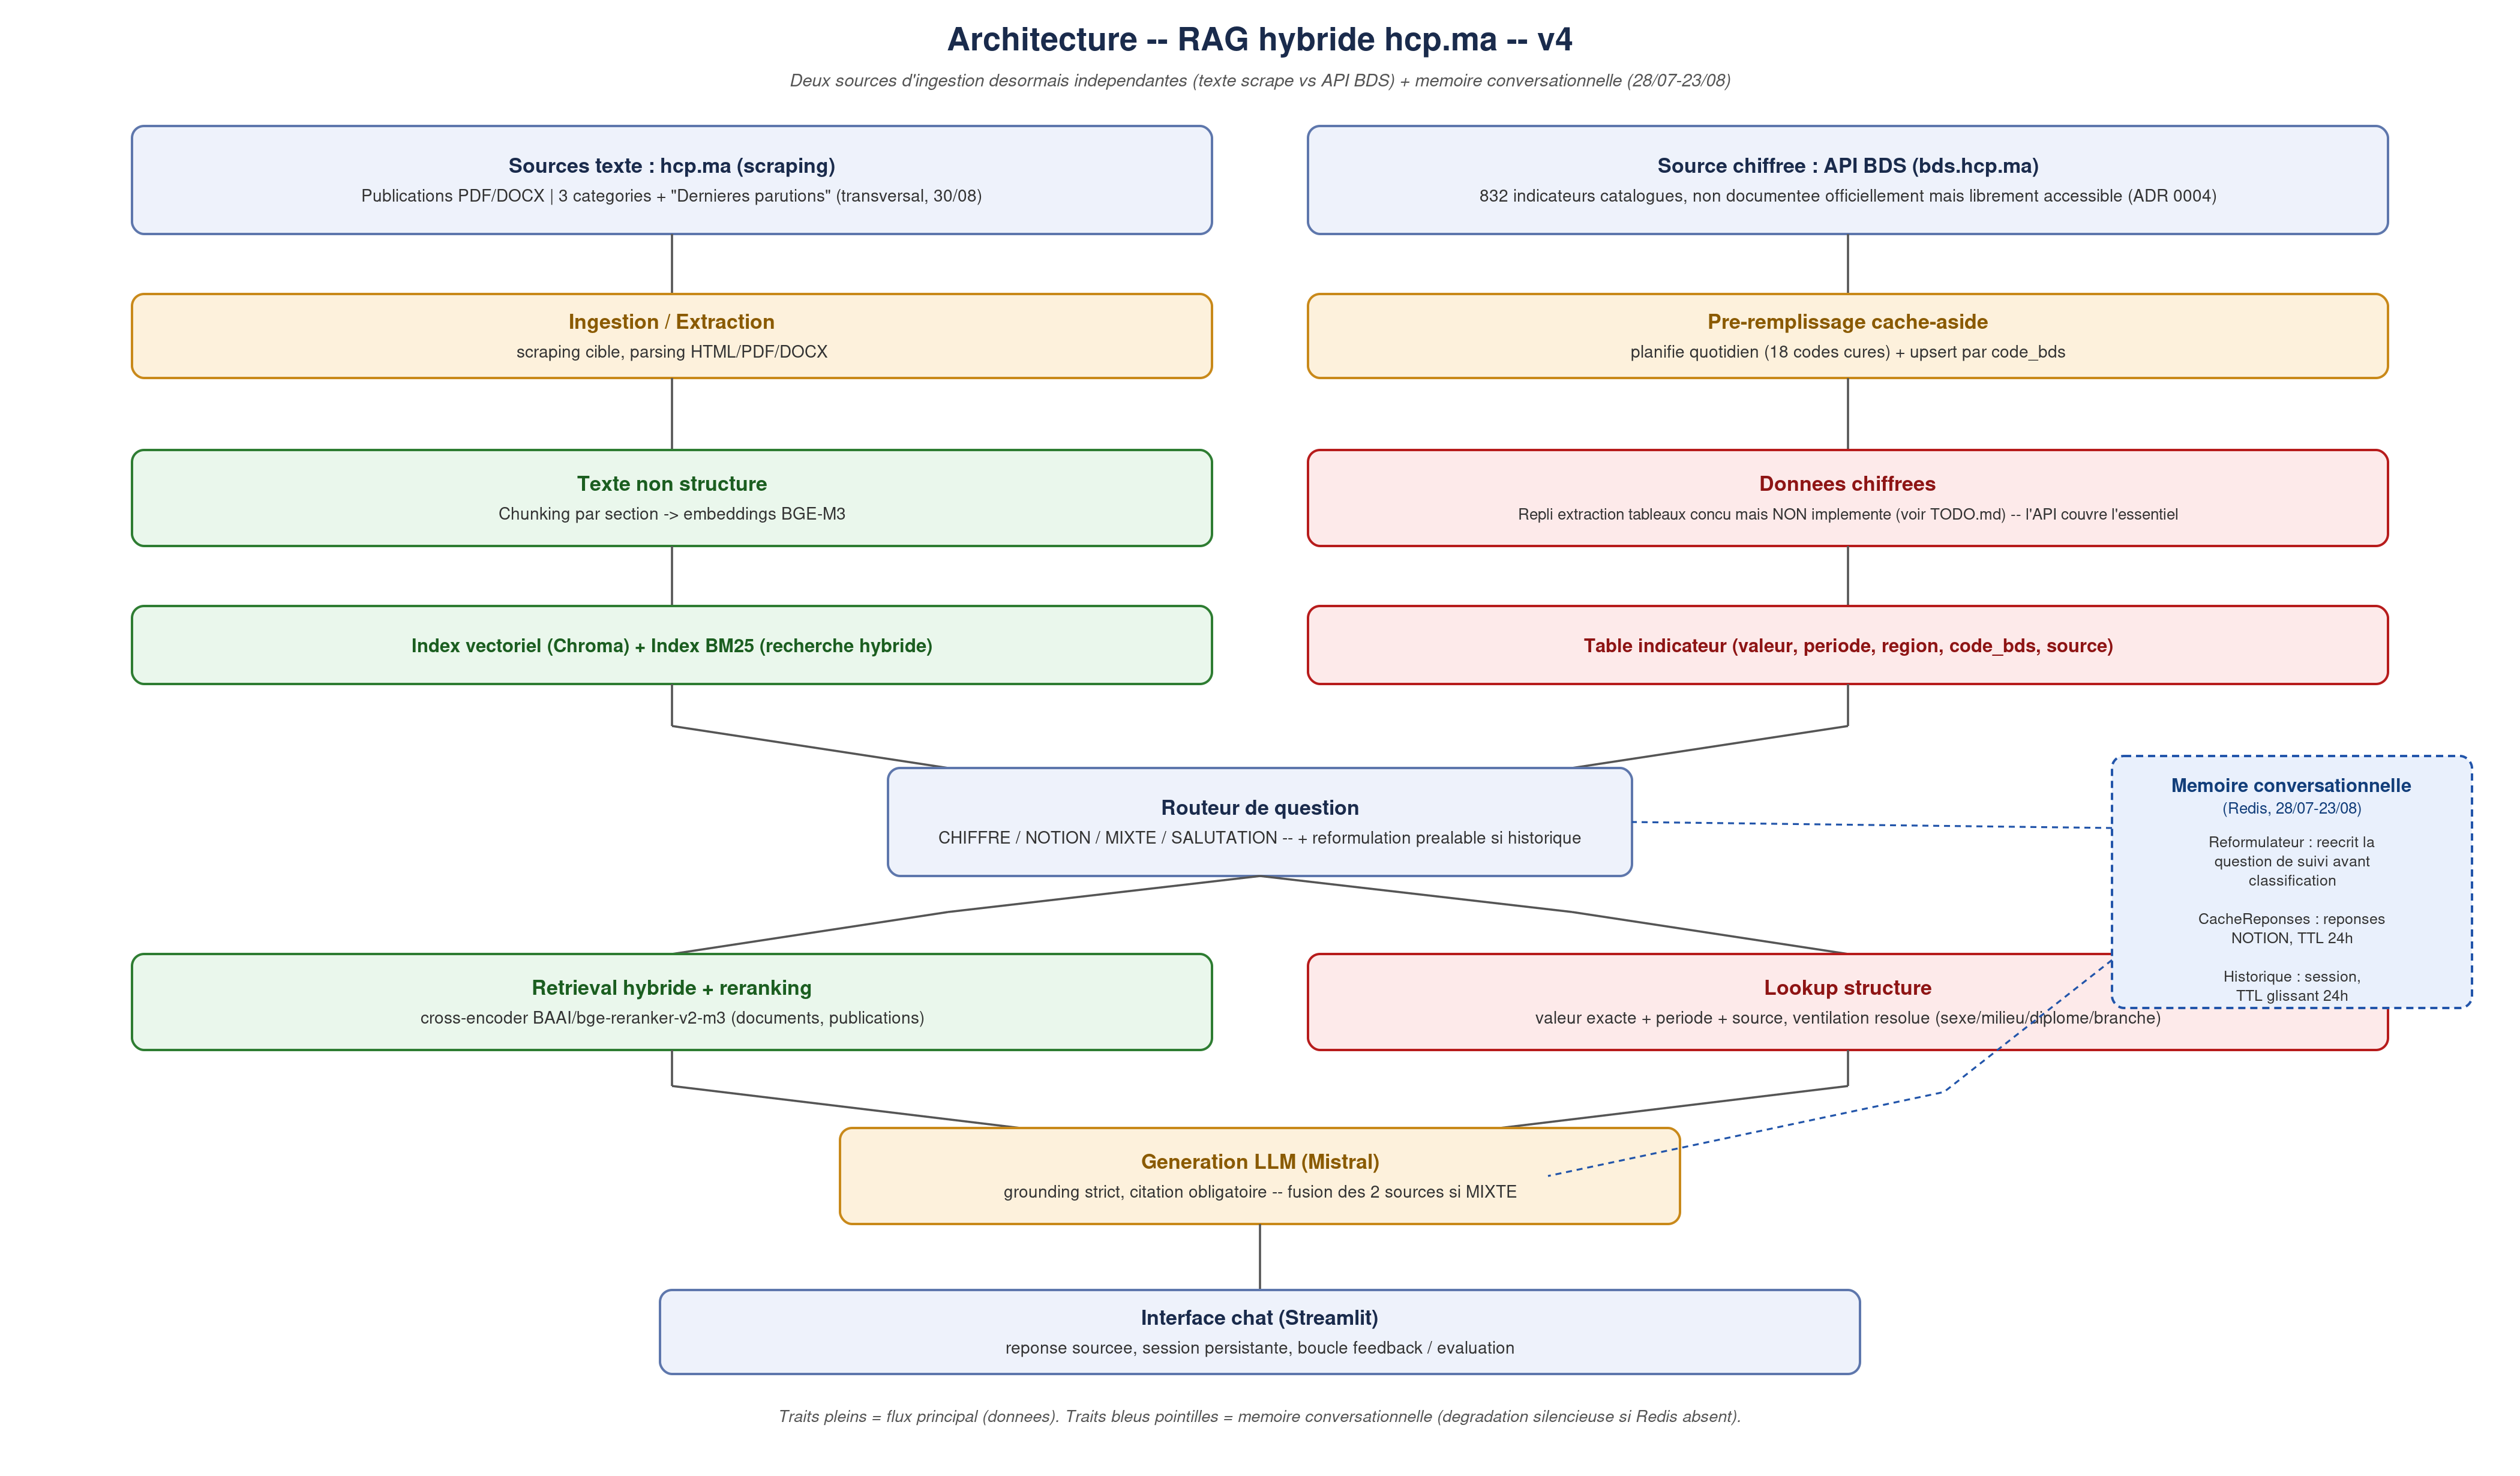
\includegraphics[width=0.75\textwidth]{images/architecture.png}
\end{figure}

\subsection{D\'etail des modules}
\begin{longtable}{@{}p{3.3cm}p{5.8cm}p{6.4cm}@{}}
\rowcolor{navy}
\tblhead{Module} & \tblhead{R\^ole} & \tblhead{Flux (entr\'ee $\rightarrow$ sortie)} \\
\midrule
\endhead
1. Scraper & Collecte les pages et PDF des cat\'egories cibl\'ees. & Liste d'URLs $\rightarrow$ fichiers bruts HTML/PDF + m\'etadonn\'ees de base \\
2. Extracteur / Parseur & Nettoie le contenu et s\'epare texte narratif et tableaux de chiffres. & Fichiers bruts $\rightarrow$ texte propre + tableaux extraits \\
3. Indexeur texte & D\'ecoupe le texte (chunking), calcule les embeddings, indexe. & Texte propre $\rightarrow$ index vectoriel + index BM25 \\
4. Constructeur base indicateurs & Structure les chiffres cl\'es extraits des tableaux. & Tableaux extraits $\rightarrow$ table indicateurs (SQL) \\
5. Routeur & Classifie la question~: chiffre pr\'ecis ou notion/narratif. & Question utilisateur $\rightarrow$ redirection module 6 ou 7 \\
6. Retrieval + reranking & Recherche hybride (sens + mots-cl\'es), puis tri de pertinence. & Question + index texte $\rightarrow$ 3 \`a 5 passages pertinents \\
7. Lookup structur\'e & Requ\^ete directe et exacte sur la table indicateurs. & Question + filtres $\rightarrow$ valeur exacte + source \\
8. G\'en\'erateur & R\'edige la r\'eponse en langage naturel avec citation obligatoire. & Passages ou valeur+source $\rightarrow$ r\'eponse finale \\
9. Interface & Affiche la question, la r\'eponse et la source cliquable. & R\'eponse finale $\rightarrow$ affichage utilisateur \\
\end{longtable}

\majcadrage{Module 4 finalement aliment\'e en priorit\'e par l'API de la Base de Donn\'ees Statistiques du HCP (\texttt{bds.hcp.ma}), et non par extraction de tableaux PDF/XLSX comme pr\'evu ici -- source non identifi\'ee au moment de la r\'edaction de cette fiche. D\'ecouverte le 15 juillet en cherchant un acc\`es plus direct aux chiffres officiels~: cette API, non document\'ee publiquement mais librement accessible, s'est av\'er\'ee plus fiable que l'extraction PDF/XLSX pour les indicateurs cur\'es. Voir ADR 0004 (\texttt{docs/adr/0004-api-bds-pour-les-indicateurs.md}). L'extraction PDF/XLSX (module 2) reste utilis\'ee pour le contenu narratif et les documents hors p\'erim\`etre de la BDS.}

\majcadrage{Le repli PDF/XLSX pour les indicateurs (envisag\'e ci-dessus comme source de secours) a finalement \'et\'e impl\'ement\'e le 3 septembre (\texttt{ConstructeurIndicateurs.structurer}), apr\`es qu'un document XLSX r\'eel d\'ej\`a collect\'e (\guillemotleft{} indicateurs trimestriels EMO \guillemotright{}) s'est av\'er\'e totalement inerte faute de ce chemin~: extraction fonctionnelle mais z\'ero indicateur ins\'er\'e en base. Reconna\^it un motif pr\'ecis (dictionnaire Code/Nom/Unit\'e + tableau de donn\'ees), test\'e sur les vraies donn\'ees (1728 lignes, valeurs exactes, aucune r\'egression sur le jeu de fiabilit\'e). Une tentative de g\'en\'eraliser \`a \emph{tout} fichier Excel du HCP a \'et\'e explor\'ee -- fichiers r\'eels t\'el\'echarg\'es et ouverts pour comparer -- puis abandonn\'ee~: l'\guillemotleft{} Annuaire Statistique du Maroc \guillemotright{} s'est av\'er\'e \^etre une archive de 23 fichiers Excel $\times$ jusqu'\`a 34 feuilles bilingues mises en page pour l'impression, sans dictionnaire ni structure programmatique -- aucun format Excel unique chez le HCP, donc pas de parseur g\'en\'erique universel s\^ur. Limite assum\'ee et document\'ee plut\^ot que contourn\'ee (voir JOURNAL.md, 03/09).}

\subsection{Mod\`ele de donn\'ees}
\begin{longtable}{@{}p{3.2cm}p{12cm}@{}}
\rowcolor{navy}
\tblhead{Table} & \tblhead{Champs principaux} \\
\midrule
\endhead
documents & id, url, titre, date\_publication, langue, categorie, type (html/pdf) \\
chunks & id, document\_id, texte du morceau, position, embedding (vecteur) \\
indicateurs & id, nom\_indicateur, valeur, unite, periode, region, document\_source \\
\end{longtable}

\subsection{Sc\'enarios d'ex\'ecution (exemples)}
\textbf{Question chiffr\'ee -- «~Quel est le taux de ch\^omage actuel~?~»~:} Interface $\rightarrow$ Routeur (d\'etecte «~chiffre~») $\rightarrow$ Lookup structur\'e dans la table indicateurs $\rightarrow$ valeur exacte + source $\rightarrow$ G\'en\'erateur r\'edige une phrase courte et sourc\'ee $\rightarrow$ Interface affiche la r\'eponse.

\textbf{Question conceptuelle -- «~C'est quoi le RGPH~?~»~:} Interface $\rightarrow$ Routeur (d\'etecte «~notion~») $\rightarrow$ Retrieval hybride dans l'index texte $\rightarrow$ Reranking garde les meilleurs passages $\rightarrow$ G\'en\'erateur r\'edige une explication sourc\'ee $\rightarrow$ Interface affiche la r\'eponse.

\subsection{Choix technologiques propos\'es}
\begin{longtable}{@{}p{5cm}p{10.2cm}@{}}
\rowcolor{navy}
\tblhead{Composant} & \tblhead{Techno propos\'ee} \\
\midrule
\endhead
Scraping & requests + BeautifulSoup \\
Extraction PDF / tableaux & PyMuPDF ou pdfplumber, Camelot pour les tableaux \\
Embeddings & Mod\`ele multilingue open source (ex.\ BGE-M3) \\
Index vectoriel & Chroma (simple \`a installer, suffisant pour un prototype) \\
Recherche mots-cl\'es & BM25 (ex.\ librairie rank\_bm25) \\
Reranking & Cross-encoder open source (ex.\ bge-reranker) \\
Base indicateurs & SQLite \\
LLM de g\'en\'eration & \`A d\'efinir -- point ouvert, voir section 11 \\
Interface de d\'emonstration & Streamlit \\
\end{longtable}

\majcadrage{Choix confirm\'es en pratique~: extraction PDF/tableaux par \texttt{pdfplumber} seul (\texttt{extract\_tables} int\'egr\'e suffisant -- PyMuPDF et Camelot, envisag\'es ici, jamais utilis\'es au final). LLM de g\'en\'eration tranch\'e le 21 juillet~: \textbf{Mistral} (\texttt{mistral-small-latest}, API externe, tier gratuit), retenu apr\`es comparaison avec Google Gemini et Groq pour la qualit\'e du fran\c{c}ais. Voir ADR 0002 (\texttt{docs/adr/0002-stack-technique-prototype.md}) pour le d\'etail de la comparaison. Le reste de la stack (BGE-M3, Chroma, rank-bm25, SQLite, Streamlit) confirm\'e sans changement.}

\subsection{Points de robustesse \`a pr\'evoir}
\begin{itemize}
\item Si le routeur se trompe de cat\'egorie, pr\'evoir un filet de s\'ecurit\'e~: si le lookup structur\'e ne trouve rien, basculer automatiquement sur le retrieval texte.
\item Si aucune source pertinente n'est trouv\'ee, la r\'eponse doit \^etre «~information non disponible dans les sources~» plut\^ot qu'une r\'eponse g\'en\'er\'ee sans base.
\end{itemize}

\section{Analyse des risques}
Les risques principaux identifi\'es \`a ce stade et leurs mesures de mitigation associ\'ees~:

\begin{longtable}{@{}p{4cm}p{2cm}p{2.2cm}p{6cm}@{}}
\rowcolor{navy}
\tblhead{Risque} & \tblhead{Impact} & \tblhead{Probabilit\'e} & \tblhead{Mitigation} \\
\midrule
\endhead
Hallucination sur un chiffre officiel & \'Elev\'e & Moyenne & S\'eparation stricte indicateurs/texte, grounding strict, citation obligatoire \\
D\'elai tr\`es serr\'e (4-5 semaines) & \'Elev\'e & \'Elev\'ee & P\'erim\`etre volontairement restreint, priorisation des fonctionnalit\'es coeur \\
Qualit\'e variable de l'extraction PDF & Moyen & Moyenne & Curation manuelle des indicateurs cl\'es en phase 1, OCR en secours \\
D\'ependance \`a une API LLM externe & Moyen & Moyenne & Clarifier avec l'encadrante, pr\'evoir repli open source \\
Contenu bilingue FR/AR complexifiant l'indexation & Faible pour le prototype & Faible (AR hors scope V1) & Fran\c{c}ais prioritaire, arabe en extension \\
\end{longtable}

\majcadrage{Risque «~qualit\'e variable de l'extraction PDF~» concr\'etis\'e~: un document r\'eellement en base (police arabe legacy) produisait des symboles bruts index\'es. Mitigation r\'eelle appliqu\'ee le 3 septembre~: garde-fou de d\'etection/exclusion (voir encadr\'e section~6), et non l'OCR envisag\'e ici -- l'OCR reste une piste document\'ee mais non impl\'ement\'ee.}

\section{Crit\`eres de r\'eussite}
\begin{itemize}
\item Le prototype r\'epond correctement, avec source cit\'ee, \`a au moins 80 \`a 90~\% des questions du jeu de test.
\item La d\'emonstration fonctionne de bout en bout sur les cat\'egories de contenu retenues.
\item Le code est versionn\'e, document\'e et reproductible par un tiers.
\item Le rapport de stage et la pr\'esentation finale sont pr\^ets avant la fin du stage.
\end{itemize}

\majcadrage{Crit\`ere de fiabilit\'e atteint et d\'epass\'e~: 93,3~\% (28/30) mesur\'e le 3 septembre, contre 80 \`a 90~\% vis\'e ici. Code versionn\'e (git, commits locaux) et suite de tests automatis\'ee \`a 224/224 \`a la m\^eme date.}

\section{Hypoth\`eses de travail et points \`a valider}
Pour ne pas bloquer l'avancement, les hypoth\`eses par d\'efaut suivantes sont retenues d\`es maintenant~; elles seront confirm\'ees ou ajust\'ees lors du prochain point avec l'encadrante.

\begin{itemize}
\item P\'erim\`etre~: on travaille sur les cat\'egories d\'efinies en section 2~; \`a confirmer ou \'elargir plus tard.
\item H\'ebergement~: on utilise une API LLM externe pour le prototype (moins de friction)~; la question de la souverainet\'e des donn\'ees sera soulev\'ee avant toute mise en production.
\item Utilisateurs~: on con\c{c}oit pour le grand public (cas le plus exigeant en clart\'e), transposable \`a un usage interne.
\item Langue~: fran\c{c}ais prioritaire pour le prototype.
\item Donn\'ees internes~: on suppose qu'aucune base d'indicateurs interne n'est disponible et on construit depuis le site public~; \`a ajuster si le contraire est confirm\'e.
\item Budget et acc\`es API~: on utilise un acc\`es de test en attendant une clarification budg\'etaire.
\item Validation~: toute r\'eponse portant un chiffre est v\'erifi\'ee manuellement pendant la phase de test.
\item Port\'ee apr\`es le stage~: prototype fig\'e livr\'e en fin de stage, mise \`a jour continue hors p\'erim\`etre.
\end{itemize}

\majcadrage{Budget/acc\`es API r\'esolu~: Mistral, tier gratuit, validation encadrante le 21 juillet (voir ADR 0002). Validation manuelle syst\'ematique compl\'et\'ee (non remplac\'ee) par une mesure automatis\'ee~: \texttt{scripts/mesurer\_fiabilite.py}, 30 questions \`a v\'erit\'e terrain ind\'ependante, ex\'ecutable \`a tout moment sans intervention manuelle.}

\section{Planning propos\'e}
Planning cibl\'e sur 5 semaines (livraison d\'ebut ao\^ut), avec une marge de s\'ecurit\'e jusqu'\`a fin ao\^ut en cas d'al\'ea.

\begin{longtable}{@{}p{1.8cm}p{2.8cm}p{11.6cm}@{}}
\rowcolor{navy}
\tblhead{Semaine} & \tblhead{Dates} & \tblhead{Objectifs cl\'es} \\
\midrule
\endhead
S1 & 7 -- 13 juil. & Validation du p\'erim\`etre, choix de la stack, script de scraping sur les cat\'egories cibl\'ees, extraction d'un \'echantillon test. \\
S2 & 14 -- 20 juil. & Pipeline d'ingestion complet (HTML + PDF + tables), constitution de la table structur\'ee des indicateurs, g\'en\'eration des embeddings et indexation. \\
S3 & 21 -- 27 juil. & Recherche hybride + reranking, routeur de question, g\'en\'eration avec citation syst\'ematique, premiers tests de bout en bout. \\
S4 & 28 juil. -- 3 ao\^ut & Interface de d\'emonstration, constitution du jeu de test (30-50 questions), mesure de fiabilit\'e, it\'eration sur les points faibles. \\
S5 & 4 -- 10 ao\^ut & Finalisation, documentation, pr\'eparation du rapport et de la d\'emonstration finale (cible de fin de projet). \\
Marge & jusqu'\`a fin ao\^ut & R\'eserve en cas de retard, ou extension (support arabe, am\'elioration interface) si le calendrier le permet. \\
\end{longtable}

\majcadrage{Calendrier r\'eellement d\'epass\'e~: la marge pr\'evue jusqu'\`a fin ao\^ut n'a pas suffi -- le jeu de test de fiabilit\'e et la finalisation (Sprint 5) n'ont \'et\'e cl\^otur\'es que le 3 septembre. \'Ecart assum\'e~: pas de r\'egression sur le p\'erim\`etre, juste un allongement de la phase de finalisation/mesure.}

\section{Glossaire}
\begin{longtable}{@{}p{4cm}p{10.2cm}@{}}
\rowcolor{navy}
\tblhead{Terme} & \tblhead{D\'efinition} \\
\midrule
\endhead
RAG (Retrieval-Augmented Generation) & M\'ethode qui r\'ecup\`ere des documents pertinents avant de g\'en\'erer une r\'eponse, pour ancrer le mod\`ele dans des sources v\'erifi\'ees plut\^ot que dans sa seule m\'emoire d'entra\^inement. \\
LLM (Large Language Model) & Mod\`ele de langage entra\^in\'e sur de grands volumes de texte, capable de comprendre et g\'en\'erer du langage naturel. \\
Embedding & Repr\'esentation num\'erique (vecteur) d'un texte qui capture son sens, permettant de comparer des textes par similarit\'e s\'emantique. \\
Chunking & D\'ecoupage d'un document en morceaux (chunks) de taille g\'er\'ee, avant indexation. \\
Index vectoriel & Base de donn\'ees sp\'ecialis\'ee dans le stockage et la recherche rapide de vecteurs (embeddings) par similarit\'e. \\
BM25 & Algorithme classique de recherche par mots-cl\'es, bas\'e sur la fr\'equence des termes. \\
Reranking & \'Etape qui retrie les documents candidats r\'ecup\'er\'es pour ne garder que les plus pertinents, \`a l'aide d'un mod\`ele plus pr\'ecis. \\
Grounding & Contrainte impos\'ee au LLM de ne r\'epondre qu'\`a partir des informations fournies dans le contexte r\'ecup\'er\'e. \\
Hallucination & G\'en\'eration par un LLM d'une information plausible mais fausse ou non v\'erifi\'ee. \\
MCD / MLD & Mod\`ele Conceptuel de Donn\'ees / Mod\`ele Logique de Donn\'ees -- repr\'esentations formelles (m\'ethode Merise) des entit\'es, attributs et relations d'une base de donn\'ees relationnelle. \\
\end{longtable}

\end{document}
